
\documentclass{beamer}
\usepackage[utf8]{inputenc}
\usepackage{amsmath}
\usepackage{amsfonts}
\usepackage{amssymb}
\usepackage{subfigure}
\usepackage{graphicx}
\usetheme{Boadilla}
\author{Mitch Davis, Kevin Burns}
\title{FOX-1 Camera Board}
\subtitle{Software Group}
\institute{Virginia Tech}
\date{Jan 2013}

\begin{document}

\section{Titlepage}
\begin{frame}
\titlepage
\end{frame}

\section{Overview}
\begin{frame}{Overview}
	\begin{itemize}
		\item Key Components
		\item Task Diagram
		\item System Operation Flowchart
		\item Programming Task List
		\item State of Development
	\end{itemize}
\end{frame}

\section{Key Components}
\begin{frame}{Key Components}
	\begin{block}{System Architecture}
		\begin{itemize}
			\item Processor: STM32L151ZDT6
			\item Operating System: ChibiOS/RT
		\end{itemize}
	\end{block}
	\begin{block}{Hardware Capabilities}
		\begin{itemize}
			\item 32MHz Processor @ 238 uA/MHz
			\item 382 KB ECC Flash, 48 KB SRAM, 12 KB ECC EEPROM
			\item 382 KB Dual-Port DRAM FIFO
			\item 1Mb 40MHz SPI MRAM
			\item 400 kHz SCCB (I2C compatible) Camera Control
			\item Two 19.2 kbaud UART
		\end{itemize}
	\end{block}
\end{frame}

\begin{frame}{Operating System}
	\begin{block}{Key Features}
		\begin{itemize}
			\item 1.2-5.5 KiB Kernel Size
			\item 128 thread priority levels
			\item Preemptive scheduling, Round-Robin schedular for like priorities
			\item Mutexes, Semaphores, Events, Message Queues
			\item Thread-safe Heap
			\item Hardware Abstraction Layer with DMA support for STM32L1
			\item GPLv3
		\end{itemize}
	\end{block}
\end{frame}

\begin{frame}{JPEG Compressor}
	\begin{block}{jpegant}
		\begin{itemize}
			\item JPEG Compressor code is based off the jpegant lightweight JPEG library
			\item Integer DCT
			\item Low memory footprint
			\item GPLv2 (Author will re-release under GPLv3 per our request)
		\end{itemize}
	\end{block}
\end{frame}

\section{Task Diagram}
\begin{frame}{Task Diagram}
	\begin{center}
%		\large{Task Diagram}
        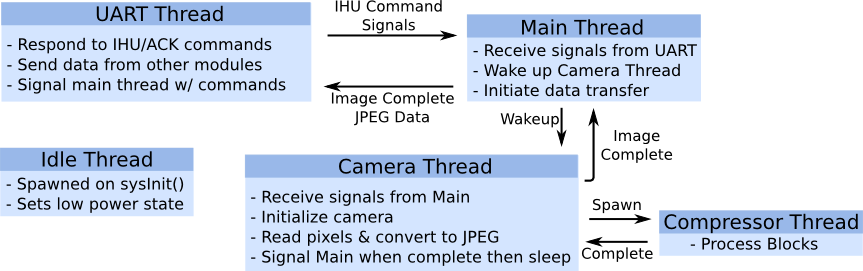
\includegraphics[scale=0.5]{task_diagram.png}
	\end{center}
\end{frame}

\section{System Operation Flowchart}
\begin{frame}{System Operation Flowchart}
	\begin{center}
%		\large{System Operation Flowchart}
        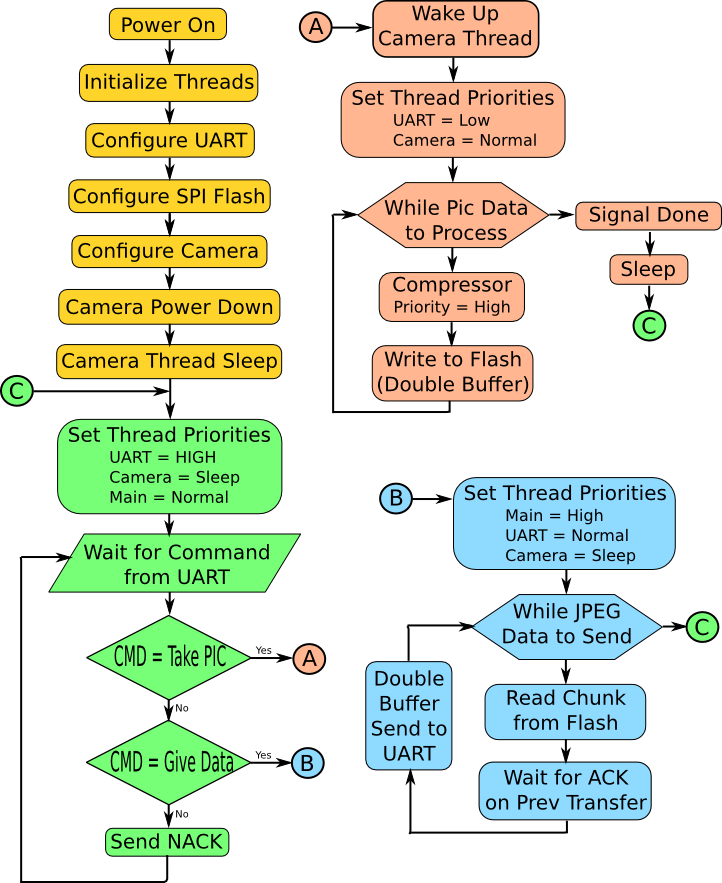
\includegraphics[scale=0.30]{flow_chart.png}
	\end{center}
\end{frame}

\section{Programming Task List}
\begin{frame}{Programming Task List}
	\begin{center}
		\large{Programming Task List}
	\end{center}
\end{frame}


\begin{frame}{State of Development}
\section{State of Development}
		\begin{itemize}
			\item STM32L152xB Development Boards received on Tuesday
			\item Existing STM32F4 code ported and runs successfully as of Tuesday
			\item OV7670 SCCB Interface is in work
			\item Need to discuss interface communications with IHU folks
		\end{itemize}
\end{frame}

\end{document}
